\section{Experiments}
\label{sec:experiments}

\subsection{Experimental Setup}
\label{sec:setup}

\paragraph{Datasets.} We evaluate on two bearing run-to-failure datasets with complementary characteristics:

\begin{table}[t]
\centering
\caption{Dataset summary. Episodes are complete run-to-failure sequences from initial operation to bearing failure.}
\label{tab:datasets}
\small
\begin{tabular}{@{}lcccccc@{}}
\toprule
Dataset & Episodes & Sampling Rate & Channels & Lifetime Range & Operating Conditions \\
\midrule
FEMTO (PRONOSTIA) & 16 & 25.6\,kHz & 1 (vibration) & 1--7\,h & 3 load/speed settings \\
XJTU-SY & 7 & 25.6\,kHz & 2 (H+V vib.) & 0.5--2.6\,h & 3 load/speed settings \\
\midrule
\textbf{Combined} & \textbf{23} &  -  &  -  & \textbf{CV=0.635} & \textbf{6 conditions} \\
\bottomrule
\end{tabular}
\end{table}

\paragraph{Evaluation protocol.} All methods are evaluated with 75\%/25\% episode-based train/test splits, fixed across methods. We report RMSE on normalized RUL ($\in [0, 1]$) averaged over 5 seeds (10 seeds for cross-dataset experiments) with standard deviations. Statistical significance is assessed via paired $t$-tests.

\paragraph{Baselines.} We compare 11 methods spanning naive baselines, end-to-end deep learning, handcrafted features, and self-supervised approaches:
\begin{itemize}[nosep]
  \item \textbf{Naive}: Constant mean predictor, elapsed-time-only baseline.
  \item \textbf{Signal processing}: Envelope RMS + LSTM.
  \item \textbf{End-to-end}: CNN-LSTM, CNN-GRU-MHA.
  \item \textbf{Handcrafted}: HC+LSTM, HC+MLP, Transformer+HC.
  \item \textbf{Self-supervised}: Random JEPA+LSTM (untrained encoder), JEPA+LSTM (pretrained).
  \item \textbf{Hybrid}: JEPA+HC Transformer (our best).
\end{itemize}

\subsection{In-Domain RUL Prediction}
\label{sec:indomain}

\begin{table}[t]
\centering
\caption{In-domain RUL prediction results (mixed FEMTO+XJTU-SY, 5-seed average). Improvement is relative reduction in RMSE vs.\ elapsed-time-only baseline (RMSE=0.224).}
\label{tab:main_results}
\small
\begin{tabular}{@{}llccc@{}}
\toprule
Category & Method & RMSE & $\pm$std & vs.\ Time-Only \\
\midrule
\multirow{2}{*}{Naive} & Constant mean & 0.290 &  -  & $-29.4\%$ \\
& Elapsed time only & 0.224 &  -  & 0\% \\
\midrule
Signal proc. & Envelope RMS + LSTM & 0.287 & 0.001 & $-28.1\%$ \\
\midrule
\multirow{2}{*}{End-to-end} & CNN-LSTM & 0.195 & 0.005 & $+13.0\%$ \\
& CNN-GRU-MHA & 0.185 & 0.005 & $+17.4\%$ \\
\midrule
\multirow{3}{*}{Handcrafted} & HC + LSTM & 0.177 & 0.016 & $+21.2\%$ \\
& HC + MLP & 0.085 & 0.004 & $+62.0\%$ \\
& Transformer + HC & 0.070 & 0.006 & $+68.9\%$ \\
\midrule
\multirow{2}{*}{Self-supervised} & Random JEPA + LSTM & 0.221 & 0.008 & $+1.5\%$ \\
& JEPA + LSTM & 0.189 & 0.015 & $+15.8\%$ \\
\midrule
\textbf{Hybrid} & \textbf{JEPA + HC Transformer} & \textbf{0.055} & \textbf{0.004} & $\mathbf{+75.5\%}$ \\
\bottomrule
\end{tabular}
\end{table}

\Cref{tab:main_results} presents the complete comparison. Several findings emerge:

\paragraph{JEPA pretraining is effective.} JEPA+LSTM (RMSE 0.189) significantly outperforms both the elapsed-time baseline ($+15.8\%$, $p = 0.010$) and random encoder initialization ($p = 0.010$). The pretrained encoder learns meaningful vibration representations without any RUL labels.

\paragraph{JEPA matches handcrafted features.} The difference between JEPA+LSTM (0.189) and HC+LSTM (0.177) is not statistically significant ($p = 0.40$), demonstrating that self-supervised pretraining can match decades of domain expertise in feature engineering - without requiring that expertise.

\paragraph{The hybrid wins decisively.} Combining JEPA embeddings with handcrafted features in a Transformer architecture achieves the best result: RMSE $0.055 \pm 0.004$, a $75.5\%$ improvement over elapsed-time and $21.4\%$ over the best handcrafted-only method (Transformer+HC at 0.070). This confirms that JEPA captures complementary information to spectral statistics.

\begin{figure}[t]
\centering
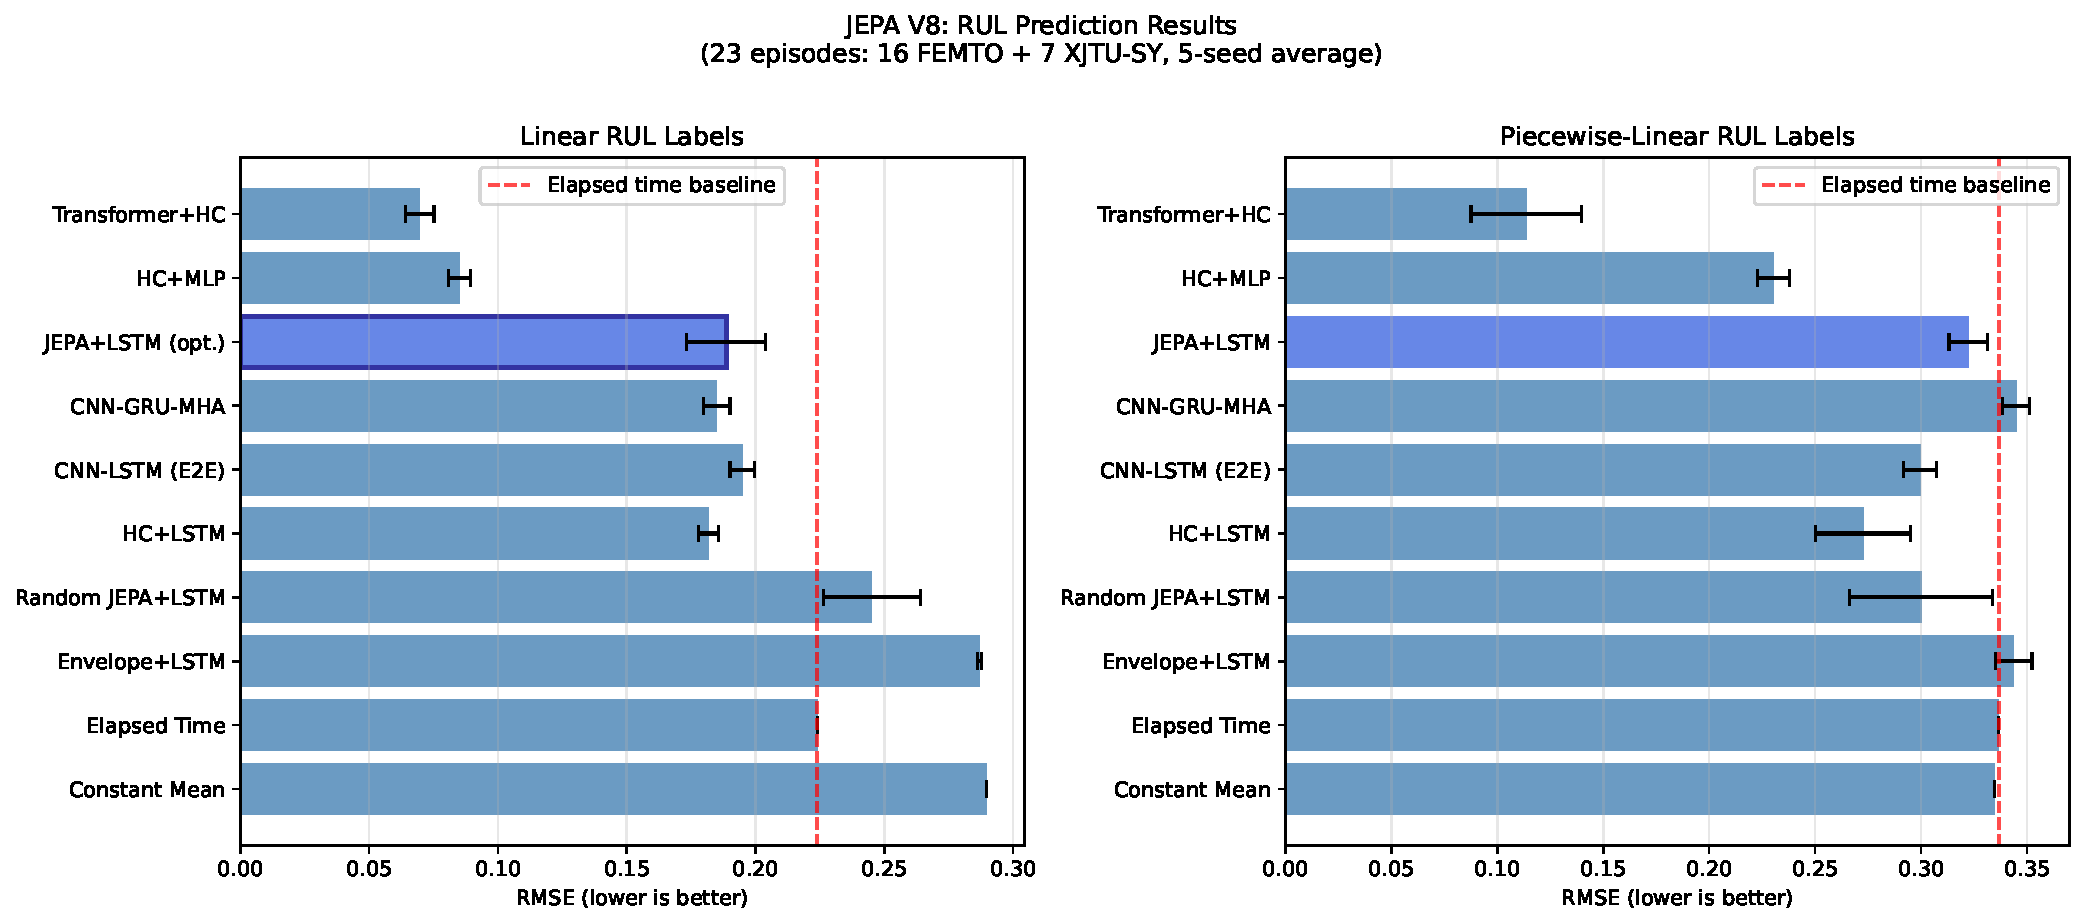
\includegraphics[width=\linewidth]{figures/v8_rul_comparison.pdf}
\caption{In-domain RUL prediction comparison across 11 methods. The hybrid JEPA+HC Transformer achieves the lowest RMSE, substantially outperforming both pure self-supervised and pure handcrafted approaches.}
\label{fig:rul_comparison}
\end{figure}

\subsection{Cross-Dataset Transfer}
\label{sec:transfer}

Cross-dataset transfer - training on one bearing test rig and evaluating on another - is the critical test of learned representations. Different test rigs have different operating conditions, bearing types, and lifetime distributions (coefficient of variation = 0.635).

\begin{table}[t]
\centering
\caption{Cross-dataset transfer results (10-seed average). Elapsed time baseline degrades sharply cross-dataset due to lifetime distribution mismatch.}
\label{tab:transfer}
\small
\begin{tabular}{@{}lcccc@{}}
\toprule
Configuration & Elapsed Time & JEPA+LSTM & Contrastive+LSTM & Contrastive vs.\ JEPA \\
\midrule
FEMTO$\to$FEMTO (within) & 0.027 & $0.113 \pm 0.011$ & $0.142 \pm 0.012$ & $-20.4\%$ \\
XJTU$\to$XJTU (within) & 0.159 & 0.195 & 0.214 & $-9.7\%$ \\
\midrule
\textbf{FEMTO$\to$XJTU (cross)} & \textbf{0.367} & $0.280 \pm 0.007$ & $\mathbf{0.227 \pm 0.015}$ & $+18.8\%$ ($p < 0.001$) \\
\textbf{XJTU$\to$FEMTO (cross)} & \textbf{0.336} & 0.403 & $\mathbf{0.309 \pm 0.007}$ & $+23.2\%$ \\
\bottomrule
\end{tabular}
\end{table}

\paragraph{Contrastive dominates cross-dataset.} Temporal contrastive learning significantly outperforms JEPA for cross-dataset transfer ($+18.8\%$ on FEMTO$\to$XJTU, $p < 0.001$). This is because the contrastive objective forces the encoder to learn what \emph{changes} over a bearing's life - the spectral centroid shift - which is the invariant degradation signature across datasets.

\paragraph{JEPA wins within-dataset.} Conversely, JEPA achieves lower RMSE within datasets, especially on FEMTO (0.113 vs 0.142). JEPA's patch prediction objective preserves fine-grained waveform details that are useful when train and test distributions match.

\paragraph{Both beat elapsed time.} In the cross-dataset setting, where elapsed time baselines degrade sharply (RMSE 0.336--0.367), both learned representations provide substantial improvement ($+24\%$ for JEPA, $+38\%$ for contrastive vs time-only).

\begin{figure}[t]
\centering
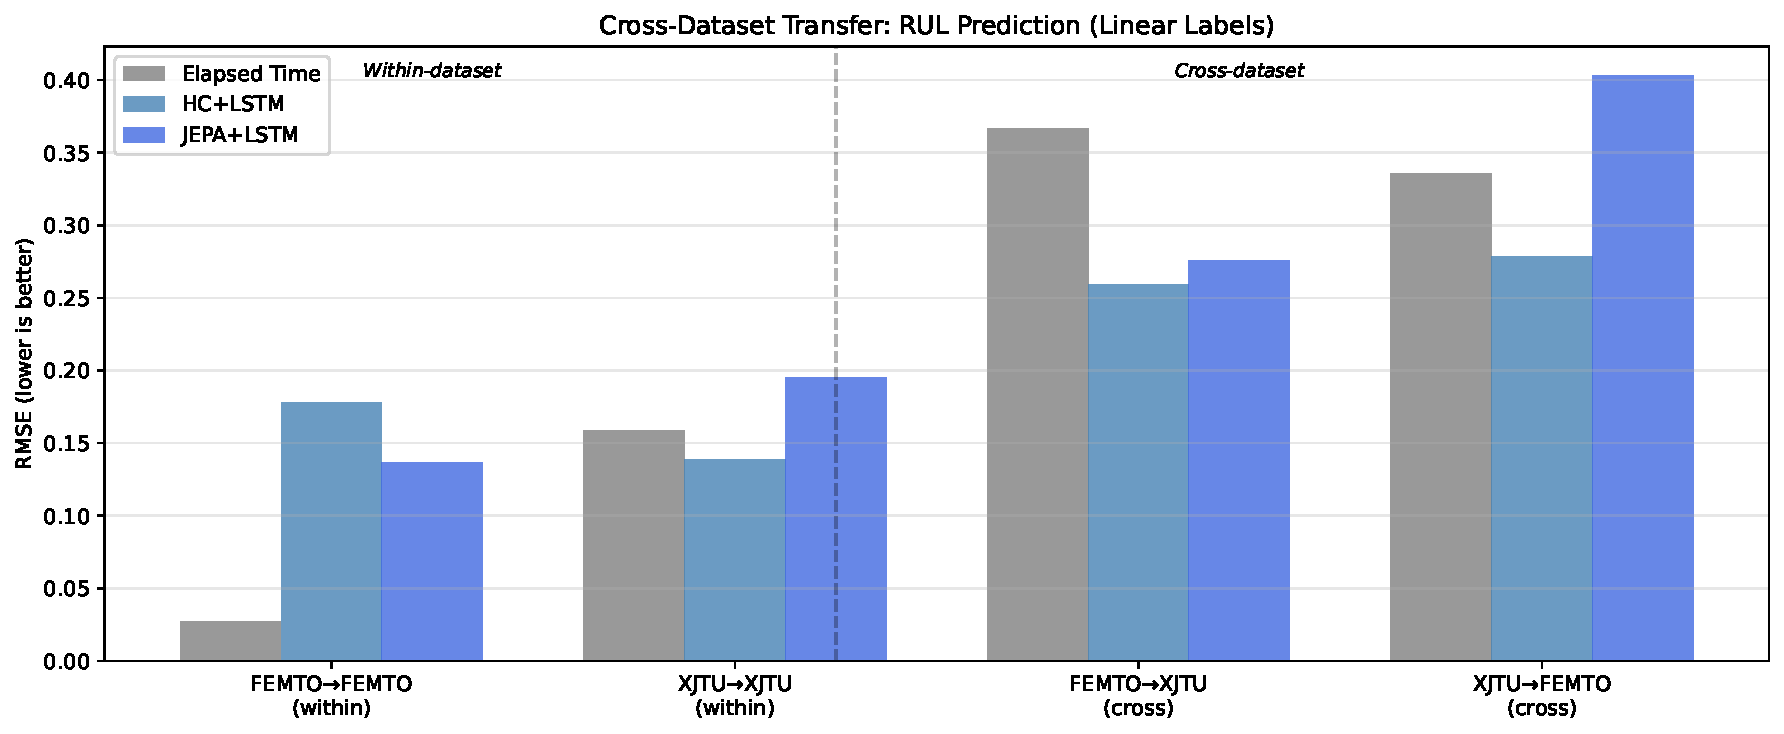
\includegraphics[width=\linewidth]{figures/v8_cross_dataset.pdf}
\caption{Cross-dataset transfer results. Temporal contrastive learning dominates when transferring across test rigs (FEMTO$\to$XJTU-SY), while JEPA is preferred within-dataset where fine-grained waveform features are discriminative.}
\label{fig:cross_dataset}
\end{figure}
